\documentclass{article}
\usepackage{amsmath}
\usepackage{graphicx}
\graphicspath{{images/}}
\title{List 1 report}
\author{Albert Kołodziejski}
\begin{document}
\maketitle
\section*{Exercise 1}

\subsection*{Description of problem:}
Main task in this exercise is to make some known floating point constants iteratively to get better understanding of theirs meaning.

\subsection*{Results:}
\begin{center}
\begin{tabular}{| c | c | c | c |}
    \hline
    & Float16 & Float32 & Float64\\ 
    \hline
    \text{eps()} & 0.000977 & 1.1920929e-7 & 2.220446049250313e-16\\
    \text{my\_eps()} & 0.000977 & 1.1920929e-7 & 2.220446049250313e-16\\
    float.h & - & 1.19209e-07 & 2.22045e-16\\
    \hline
    \text{nextfloat()} & 6.0e-8 & 1.0e-45 & 5.0e-324\\
    \text{my\_eta()} & 6.0e-8 & 1.0e-45 & 5.0e-324\\
    \hline
    \text{floatmax()} & 6.55e4 & 3.4028235e38 & 1.7976931348623157e308\\
    \text{my\_max()} & 6.55e4 & 3.4028235e38 & 1.7976931348623157e308\\
    float.h & - & 3.40282e+38 & 1.79769e+308\\
    \hline
\end{tabular}
\end{center}
\subsection*{QA:}
\begin{center}
    \textbf{How macheps relate to precision of arithmetic?}
\end{center}
Precision of arithmetic is a upper bound of realative error,\\
eps = 2\textsuperscript{-t}. \\
Macheps is distance to next bigger number representet in that arithmetic.\\
macheps = 2\textsuperscript{-(t - 1)}
\begin{center}
    macheps = 2\textsuperscript{-(t - 1)} = 2\textsuperscript{-t + 1} = 2\textsuperscript{-t} * 2 = eps * 2
\end{center}

\begin{center}
    \textbf{What is the relationship between the number eta \\
    and the number MIN\textsubscript{sub}?}
\end{center}
MIN\textsubscript{sub} is smallest subnormal number that can be represented. Subnormal means that it mantissa starts with 0 instead of 1. Eta is next number after zero. Both are the same. In my results it is hard to see becouse julia rounds those number, if we would take bits of both number we would see that they are the same.
\begin{center}
    \textbf{What does the function floatmin() return \\
     and what is the relationship of with MIN\textsubscript{nor}?}
\end{center}
\text{floatmin()} returns minimal normalized nummber, so it is equal to MIN\textsubscript{nor}.

\subsection*{Interpretation and conclusions:}
Naming conventions are here a little tricky, machine epsilon is not epsilon and there are 2 completely different minimal values, so better check it before blindly running floatmin() in any language.

\section*{Exercise 2}

\subsection*{Description of problem:}
Test Khan formula that may compute machine epsilon.

\subsection*{Results:}
\begin{center}
    \begin{tabular}{| c | c | c | c |}
        \hline
        & Float16 & Float32 & Float64\\ 
        \hline
        \text{experiment()} & -0.000977 & 1.1920929e-7 & -2.220446049250313e-16\\
        \text{eps()} & 0.000977 & 1.1920929e-7 & 2.220446049250313e-16\\
        \hline
    \end{tabular}
    \end{center}

\subsection*{Interpretation and conclusions:}
We can get epsilon from this formula, but if numbers of bit used for mantissa is odd we will get negativ value. There are tricky ways you can play with float arithmetic to get what you want.


\section*{Exercise 3}

\subsection*{Description of problem:}
Test how numbers are distributed in float arithmetic.

\subsection*{Results:}

\begin{center}
    \begin{tabular}{| c | c |}
        \hline
        1 + 0step & 0011111111110000000000000000000000000000000000000000000000000000\\ 
        \hline
        1 + 1step & 0011111111110000000000000000000000000000000000000000000000000001\\
        \hline
        1 + 2step & 0011111111110000000000000000000000000000000000000000000000000010\\
        \hline
        1 + 3step & 0011111111110000000000000000000000000000000000000000000000000011\\
        \hline
        1 + (2\textsuperscript{52}-2)step & 0011111111111111111111111111111111111111111111111111111111111110\\
        \hline
        1 + (2\textsuperscript{52}-1)step & 0011111111111111111111111111111111111111111111111111111111111111\\
        \hline
        1 + 2\textsuperscript{52}step & 0100000000000000000000000000000000000000000000000000000000000000\\
        \hline
    \end{tabular}
    \end{center}
Adding 1 to the end of mantissa should create all numbers between 1 and 2
\subsection*{QA:}

\begin{center}
    \textbf{How numbers are distributed in [0.5, 1] and how can be represented?}
\end{center}
They are distributed evenly with step = 2\textsuperscript{-53}, they can be represented as\\
x = 0.5 + k*step, where k = 1, 2, ..., 2\textsuperscript{51} - 1

\begin{center}
    \textbf{How numbers are distributed in [2, 4] and how can be represented?}
\end{center}
They are distributed evenly with step = 2\textsuperscript{-51}, they can be represented as\\
x = 2 + k*step, where k = 1, 2, ..., 2\textsuperscript{51} - 1

\subsection*{Interpretation and conclusions:}
Normalized numbers are distributed evenly between two neighbor powers of 2, the farther from range [1, 2] you are, the smaller amount of numbers distributed.

\section*{Exercise 4}
\subsection*{Description of problem:}
Find smallest number bigger then that breaks 1 * (1/x) = 1 formula in Float64 arithmetic.

\subsection*{Results:}
1.000000057228997

\subsection*{Interpretation and conclusions:}
Never use equal sign when dealing with float arithmetic becouse it can be counter-intuitive.

\section*{Exercise 5}
\subsection*{Description of problem:}
Find best way to compute scalar product when vectors are almost perpendicular.

\subsection*{Results:}
\begin{center}
    \begin{tabular}{| c | c | c | c |}
        \hline
         & result & error & relative error\\ 
        \hline
        forward Float32 & -0.4999443 & 0.49994429944939167 & 4.967e10\\
        backward Float32 & -0.4543457 & 0.4543457031149343 & 4.514e10\\
        ascending on Float32 & -0.5 & 0.4999999999899343 & 4.967e10\\
        descending Float32 & -0.5 & 0.4999999999899343 & 4.968e10\\
        \hline
        forward Float64 & 1.0251881368296672e-10 & 1.1258452438296671e-10 & 11.18 \\
        backward Float64 & -1.5643308870494366e-10 & 1.4636737800494365e-10 & 14.54 \\
        ascending on Float64 & 0.0 & 1.0065710699999998e-11 & 1.0 \\
        descending Float64 & 0.0 & 1.0065710699999998e-11 & 1.0\\
        \hline
    \end{tabular}
    \end{center}

\subsection*{Interpretation and conclusions:}
There is no good solutions, one can only prey to god that they are not perpendicular.

\section*{Exercise 6}
\subsection*{Description of problem:}
Check what effect avoiding subtracting 2 almost the same numbers can have on results.

\subsection*{Results:}
This formula should never reach zero for any x bigger then zero. Good check would be finding biggest i, that for x = 8\textsuperscript{-i} function is still bigger then zero.

\begin{center}
    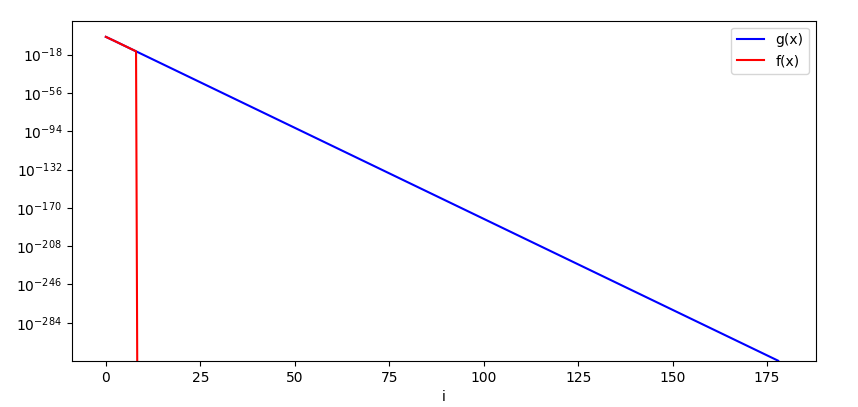
\includegraphics[scale=0.6]{f_and_g_functions} 
\end{center}

\begin{center}
    \begin{tabular}{| c | c | c |}
        \hline
         & f(x) & g(x)\\ 
        \hline
        i = 1 & 0.0077822185373186414 & 0.0077822185373187065\\
        \hline
        i = 8 & 1.7763568394002505e-15 & 1.7763568394002489e-15\\
        \hline
        i = 9 & 0.0 & 2.7755575615628914e-17\\
        \hline
        i = 178 & 0.0 & 1.6e-322\\
        \hline
        i = 179 & 0.0 & 0.0\\
        \hline
    \end{tabular}
    \end{center}
    \subsection*{QA:}

    \begin{center}
        \textbf{Although f() and g() give different results, which we should trust more?}
    \end{center}
    As we can see g() stays non zero for much longer, so we should trust it more.

    \subsection*{Interpretation and conclusions:}
We should try to avoid subtracting 2 numbers that are close to each other by reformulating.

\section*{Exercise 7}
\subsection*{Description of problem:}
Test behaviour of function that is supose to approximate derivative at the point in Float64 arithmetic.

\subsection*{Results:}
For h:
\begin{center}
    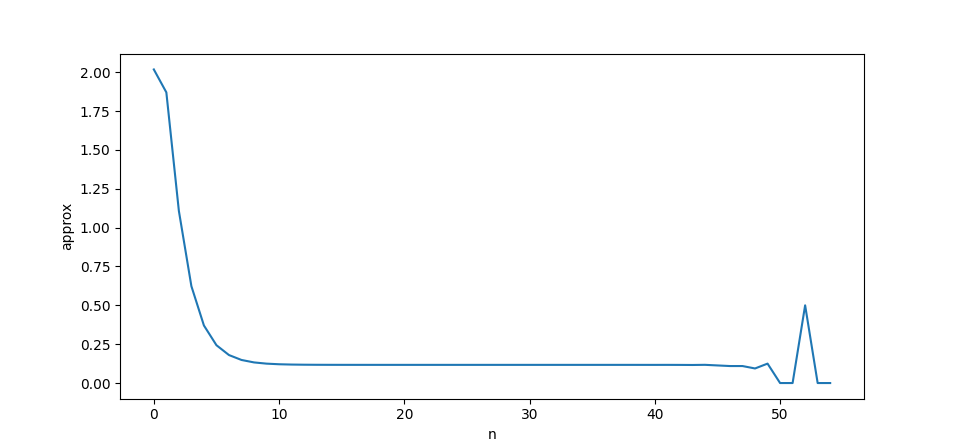
\includegraphics[scale=0.5]{h_approximation} 
    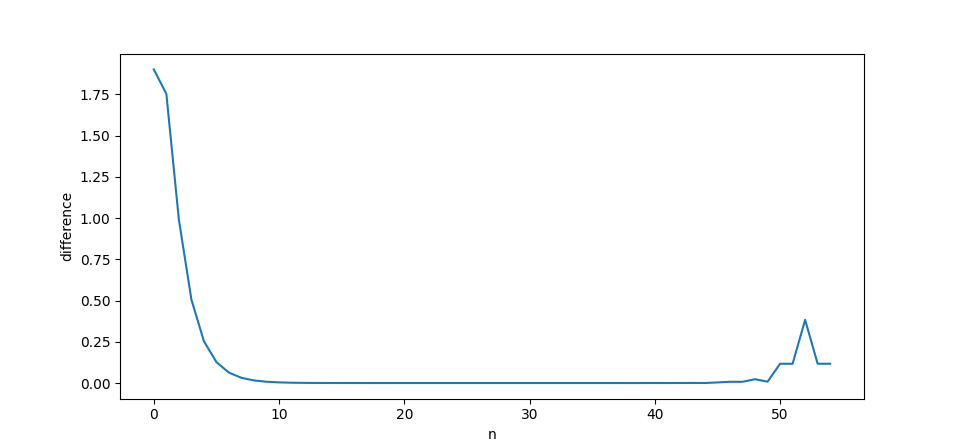
\includegraphics[scale=0.5]{h_difference} 
\end{center}

For 1 + h:
\begin{center}
    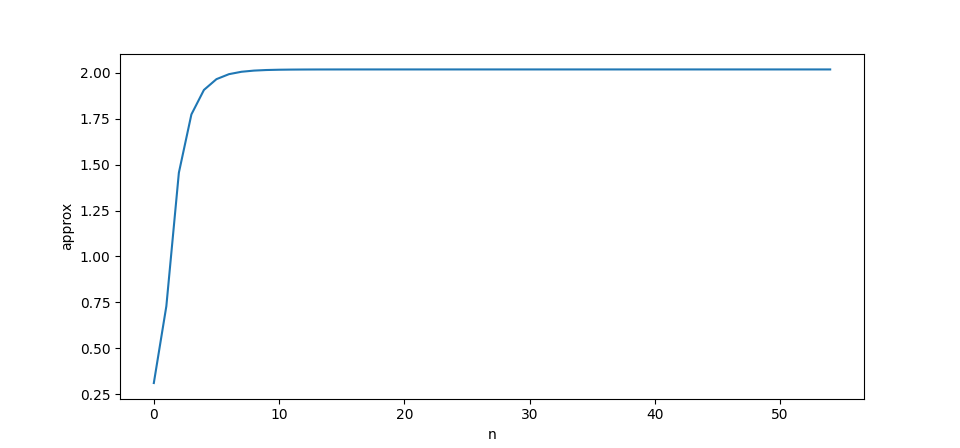
\includegraphics[scale=0.5]{h_plus_1_approximation} 
    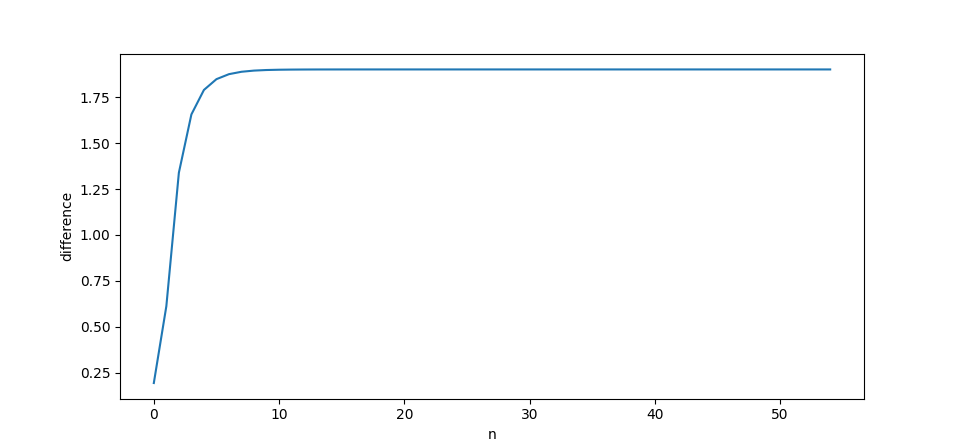
\includegraphics[scale=0.5]{h_plus_1_difference} 
\end{center}

\subsection*{QA:}

\begin{center}
    \textbf{How to explain that, from a certain point onwards, decreasing \\
    the value of h does not improve the approximation of the of \\
    the derivative?}
\end{center}
To check whats going on here we can approximate error of this calculation.
\[
    \begin{array}{c}
        \frac{sin(1+h) + cos(3+3h)(1 + \delta\textsubscript{a} +\delta\textsubscript{p}) - sin(1) - cos(3)}{h} \leq\\
        \\
        \leq\frac{sin(2) + cos(6)(1 + \delta\textsubscript{a} +\delta\textsubscript{p}) - sin(1) - cos(3)}{h}\leq\\
        \\
        \leq\frac{1}{h}(0.013 + \delta\textsubscript{a} +\delta\textsubscript{p})
    \end{array}
\]
From my computations we can see that there is huge constants that influance final result drasticly. What's more we can check for for what n, h is smaller then this error.

\[
    \log\textsubscript{2}{0.013} \approx -6.27
\]
Which correspond to the graph becouse after i = 6 there is a little change in approximation.
\begin{center}
    \textbf{How does 1 + h behave?}
\end{center}
It is not a good approximation in it self but it isn't getting worse with bigger n. Difference is always bigger then one, and similary after some point approximation stops getting better.

\end{document}